% \documentclass[preprint,12pt]{elsarticle}

%% Use the option review to obtain double line spacing
%% \documentclass[authoryear,preprint,review,12pt]{elsarticle}

%% Use the options 1p,twocolumn; 3p; 3p,twocolumn; 5p; or 5p,twocolumn
%% for a journal layout:
\documentclass[final,1p]{elsarticle}
%% \documentclass[final,1p,times,twocolumn]{elsarticle}
% \documentclass[final,3p,times]{elsarticle}
% \documentclass[final,3p,times,twocolumn]{elsarticle}
% \documentclass[final,5p,times]{elsarticle}
%% \documentclass[final,5p,times,twocolumn]{elsarticle}

%% For including figures, graphicx.sty has been loaded in
%% elsarticle.cls. If you prefer to use the old commands
%% please give \usepackage{epsfig}

%% The amssymb package provides various useful mathematical symbols
\usepackage{amssymb}
\usepackage{amsmath}
\usepackage{color}
\usepackage{hyperref}

\usepackage{minted} % First pip install pygments
\setminted{breaklines, framesep=2mm, fontsize=\footnotesize, numbersep=5pt}

%% The amsthm package provides extended theorem environments
\usepackage{amsthm}

%% The lineno packages adds line numbers. Start line numbering with
%% \begin{linenumbers}, end it with \end{linenumbers}. Or switch it on
%% for the whole article with \linenumbers.
%% \usepackage{lineno}

\journal{Github}

\newtheorem{remark}{\bf Remark}[section]
% Color codes
\newcommand{\red}[1]{{\color{red}  #1}}
\newcommand{\blue}[1]{{\color{blue}  #1}}
\newcommand{\green}[1]{{\color{green}  #1}}

\begin{document}

\begin{frontmatter}

%% Title, authors and addresses

%% use the tnoteref command within \title for footnotes;
%% use the tnotetext command for theassociated footnote;
%% use the fnref command within \author or \address for footnotes;
%% use the fntext command for theassociated footnote;
%% use the corref command within \author for corresponding author footnotes;
%% use the cortext command for theassociated footnote;
%% use the ead command for the email address,
%% and the form \ead[url] for the home page:
%% \title{Title\tnoteref{label1}}
%% \tnotetext[label1]{}
%% \author{Name\corref{cor1}\fnref{label2}}
%% \ead{email address}
%% \ead[url]{home page}
%% \fntext[label2]{}
%% \cortext[cor1]{}
%% \affiliation{organization={},
%%             addressline={},
%%             city={},
%%             postcode={},
%%             state={},
%%             country={}}
%% \fntext[label3]{}

\title{
BBB-FLIDS Project Report\\
{\small Blockchain-Based Federated Learning for Intrusion Detection}
}

%% use optional labels to link authors explicitly to addresses:
%% \author[label1,label2]{}
%% \affiliation[label1]{organization={},
%%             addressline={},
%%             city={},
%%             postcode={},
%%             state={},
%%             country={}}
%%
%% \affiliation[label2]{organization={},
%%             addressline={},
%%             city={},
%%             postcode={},
%%             state={},
%%             country={}}

\author{İlker Işık}
\ead{iiilker99@gmail.com}
%\affiliation[inst1]{organization={2380517}}
%,
%            addressline={Address One}, 
%            city={City One},
%            postcode={00000}, 
%            state={State One},
%            country={Country One}}


\begin{abstract}
In this project, I implemented a federated-learning intrusion detection system based on blockchain technology, which becomes increasingly more common in the modern world.
Since I designed a machine learning based intrusion detection system instead of a signature based one, this system has the potential to detect new attack types.
Federated learning approach allows us to ensure the privacy of the sensitive data while learning from it, and leverage the large amounts of data distributed in the client devices.
I used the federated averaging approach in conjunction with a custom preprocessing stage for data standardization.
By combining blockchain and federated learning, I created a fully open and decentralized learning system in order to overcome novel security challenges.
\end{abstract}


\begin{keyword}
%% keywords here, in the form: keyword \sep keyword
Machine Learning \sep Federated Learning \sep Blockchain
\end{keyword}

\end{frontmatter}

%% \linenumbers


\section{Introduction}
With the rapid increase in computing power, machine learning (ML) became a technique applied to almost every problem that satisfies the condition of having the necessary amount of data. In many ML applications, massive amount of user data is collected to train the ML model and get highly accurate results. Most of the applications store user data in their servers; however, this approach has problems in the sense that collecting massive amount of data is costly in terms of computation and network resources, and the collected data may include sensitive information of users, who may hesitate to share that information.

Most of the intrusion detection systems use well-known signatures of the attack vectors while classifying malicious users according to their actions. Although this approach might work well for attack vectors which are previously investigated by cyber-security experts, it cannot accurately detect new attack vectors, such as zero day attacks. In order to address this problem, statistics or ML based approaches are used, namely anomaly-based intrusion detection systems. As explained above, ML based IDS require training data from users and thus have problems about privacy.

A new ML model called federated learning was developed in order to solve problems previously explained. Federated learning (FL) is a technique where multiple clients, each having their own private data, cooperate in order to train a machine learning model \citep{bcflsurvey}.
%Clients make local updates to the model using their private data, and these updates are then combined to obtain a global model, without requiring sharing of the data.
Horizontal FL uses different samples with the same feature space and characteristics in each client.
Whereas in vertical FL, clients use the same samples with different feature space during local training.

Although FL models solve privacy related problems mentioned above, it still uses a centralized server for storing the learning results. Therefore, it is susceptible to single point of failure. In order to solve this issue, a blockchain based FL system is developed so that the system has more distributed structure and the security of the system is improved.

\section{Related Work}

Performance comparison of different FL algorithms are carried out in \cite{FLperf}, and federated averaging attained the highest accuracy.
However, it has also been shown that FL suffers when the data is non-IID (non-Independent and identically Distributed).
To overcome this, \cite{FL-HC} proposes a hierarchical clustering idea.

A fairly comprehensive literature survey about FL for intrusion detection systems (IDS) is provided in \cite{FLforIDSsurvey}.
A more general survey is given in \cite{IDSusingMLsurvey}, concerning IDS using machine learning.
These papers also provide lots of background information on IDS, which I will omit for the sake of brevity.

When the training data is scarce, anomaly detection systems deliver lots of false positives and exhibit bad performance overall.
Federated learning enables us to leverage the private data distributed in numerous devices without sharing the data directly.
For example, in the collaborative IDS presented in \cite{ColabIDS}, FL is employed in combination with a semi-supervised learning algorithm to mitigate the data scarcity issues.
Similarly, in \cite{FLwirelessIDS}, the privacy-preserving properties of FL are exploited in order to preserve sensitive data during model training.

Furthermore, due to its simplicity, federated learning offers an elegant and flexible framework for building unique machine learning applications.
A single deep neural network is trained for multiple IDS tasks in \cite{mt-dnn-fl} using FL, which even surpassed some models dedicated to a single task.
An example of using blockchain in combination with machine learning is given in \cite{dbf}, which presents a Deep Blockchain Framework for collaborative IDS.


\section{Methodology}

\subsection{Machine Learning Model}

I decided to work with neural networks in this project due to their flexibility.
The architecture of the neural network can be customized easily with a simple yet expressive configuration system.
In the results section, I will test the accuracy of the algorithm with different configurations.
The last layer will always have $L$ neurons, outputting the confidence values for $L$ classes.
After that, cross-entropy loss function is used to compare against the ground truth.

I used horizontal federated learning, i.e., all clients have different training samples with the same feature space, because I believe this is a more common use case in practical applications.

The core federated learning idea is presented in \cite{comef-FL}, which is one of the most influential papers in this field.
In this paper, the authors advocate a learning strategy in which the clients make local updates to the model, and the server averages these updates to finalize a round.
This process is called \textit{federated averaging}.
The overall strategy resembles stochastic gradient descent.

Let $w^k_t$ denote the model parameters for client $k$ at time $t$.
Similarly, $w_t$ denotes the global model parameters.
At each round, the clients perform a local update on their weights individually:
\begin{equation}
    w^k_{t+1} \leftarrow w^k_{t} - \eta \triangledown l(w^k_t)
\end{equation}
where $\eta$ is the learning rate, $l$ the loss function (computed on the local dataset), and $\triangledown l$ is its gradient w.r.t model parameters.
Since the updates done by each client are independent from each other, they can easily work in parallel.
Furthermore, each client can perform this parameter update step multiple times.
A single pass through the local dataset is termed \textit{local epoch}.
%This number is represented by the hyperparameter $E$, also known as the local epoch.

Instead of doing local updates with all clients at each round, the authors of \citep{comef-FL} introduce another hyperparameter $C$, and only perform local updates in $C$-fraction of clients at each round.
$C$ acts a bit like a global batch size in this case; $C = 1$ means all clients perform updates, therefore all of the data is utilized at each round, with smaller $C$ values reducing this amount.
The impact of changing $C$ will be evaluated in the results section.

After the local updates are completed, server averages them in order to update the global model parameters:
\begin{equation}
    w_{t+1} = \sum_{k=1}^K \frac{n_k}{n} w^k_{t+1}
\end{equation}
where $n_k$ is the amount of local data in $k$th client, and $n$ is the total, i.e., $n = \sum_{k=1}^K n_k$.
$K$ represents the total number of clients.
This concludes a single round of federated learning.
In the following round, the clients will fetch the averaged global model and perform gradient descent on it again.

I chose \verb|pytorch| and \verb|numpy| libraries to implement this machine learning model in Python because of my pre-existing familiarity with these tools.
To read the dataset, I used \verb|pandas| library.
\verb|sklearn| is also used for some preprocessing steps (e.g. converting categorical data to one-hot vectors).



\subsection{Data Standardization}

With \textit{data standardization}, I refer to the preprocessing step in which we eliminate the varying means and standard deviations of different features in the dataset.
This process is particularly important when the features have wildly different scales, e.g., one feature has a mean of $10000$ and the other $0.001$.
In fact, data standardization is deemed ``necessary" when a non-linear activation function is utilized \citep{standardizationANN}.
Intuitively, non-standardized values are less likely to trigger the non-linear response of an activation function, e.g., ReLU is linear for all positive numbers.

In a regular machine learning application, we usually remove the mean and divide the result by the standard deviation for each feature.
In literature, this is commonly known as Z-score:
\begin{equation}
    z = \frac{x - \mu}{\sigma}
\end{equation}

Unfortunately, data standardization is not studied in the federated learning paper \cite{comef-FL}, presumably because it mainly targets image data, which is already normalized.
Likewise, I failed to find any research about this issue in the literature.
However, standardization is a crucial step in this application, as I will demonstrate in results section.
Moreover, I aimed to make this project more general-purpose by not making any assumptions about the data.

My solution to data standardization in federated learning is based on the local update and general averaging steps explained in the previous section.
Before the training process starts, server and clients participate in 2 sequential preprocessing stages for data standardization, one for mean and the other for standard deviation.

Similar to the local update step, the clients report their local means to the server first, $\mu_k$ for each client $k$, alongside their data size $n_k$.
After that, the overall mean is computed by the server using the formula:
\begin{equation}
    \mu = \frac{\sum_{k=1}^K n_k \mu_k}{n}
\end{equation}
This computed $\mu$ will be used by all clients to standardize their data.
A similar process is carried out for standard deviation.
An important detail is that each client uses the global $\mu$ while computing their local standard deviation instead of the local $\mu_k$. 
\begin{align}
    \sigma_k & = \sqrt{\frac{\sum_{i=1}^{n_k} (x_i - \mu)^2}{n_k}} \\
    \sigma & = \sqrt{\frac{\sum_{k=1}^{K} n_k \sigma_k^2}{n}}
\end{align}

Also note that these two standardization steps must be done for each feature.
However, thanks to vectorized operations, this does not require a separate pass for each feature.
In practice, $\mu$, $\mu_k$, $\sigma$ and $\sigma_k$ are actually vectors of values computed for all features, e.g., $\mu_k = [\mu_{k, 1}, \mu_{k,2}, \ldots]$.


\subsubsection{Impact on Privacy}

One of the primary motivations for federated learning is to preserve the privacy of sensitive data, which is achieved by performing the updates locally and averaging them.
A stochastic gradient descent update tells very little about the training data.
However, the mean and standard deviation preprocessing steps I introduced require the clients to send the means and standard deviations of their local data, which arguably exposes more sensitive information compared to gradient descent updates.

Similar to how only a fraction of clients participate in each round of gradient descent, we can limit the participation to volunteers in these 2 preprocessing stages.
We will call this fraction $C_{pre}$.
With this approach, $\mu$ and $\sigma$ values we compute will not be exactly correct, but they will provide a reasonable estimate which is adequate in most cases.

Furthermore, in real life, dataset sizes of different clients are unlikely to be the same.
When a client hoards a large amount of data, they will have less privacy concerns about sharing the mean and standard deviation information, because these values tell a lot less about the individual data samples when the dataset size is large.
This is quite convenient for us, since $\mu_k$ and $\sigma_k$ values shared by these clients also have a larger impact on the global $\mu$ and $\sigma$.

An alternative solution is simply to ditch the standardization for the sake of privacy.
I will investigate the effect of this choice in the results section.


\subsection{Blockchain}

My primary target blockchain is Ethereum due to its popularity and good tooling support.
Consequently, I chose the Solidity programming language for the smart contract.

For interacting with the Ethereum blockchain, \verb|web3.py| library provides a clean Python interface.
Since it would be quite costly to run this project on the real Ethereum network, I made use of \verb|eth-tester| tool suite to run the project.

Furthermore, I implemented this blockchain platform in a modular manner.
In code, \verb|EthPlatform| module is responsible for communicating with the Ethereum ecosystem, which can easily be replaced due to this flexible structure.
For example, I provide a \verb|DummyPlatform| module which can emulate the functions of the previous module without interacting with an actual blockchain.
This allows us to bypass the run-time performance cost of blockchain.
Besides, this module can be beneficial to the users who want to test only the federated learning part without installing any blockchain libraries.

In Solidity, the state of the model is represented as bytes, which is obtained by combining all parameters of the model in IEEE 754 floating point representation and getting the corresponding byte representation.
Afterwards, we can use this byte data by interpreting the byte buffer as an array with correst data type and shape.
Figure \ref{fig:modelBytes} demonstrates this in Python.

\begin{figure}[h]
    \begin{minted}{python}
    # Model to bytes
    bytestr = b''
    for param in model1.parameters():
        bytestr += param.detach().numpy().tobytes()
    
    # Bytes to model
    for param in model2.parameters():
        arr = param.detach().numpy()
        arr[:] = np.frombuffer(bytestr[:arr.nbytes], dtype=arr.dtype).reshape(arr.shape)
        bytestr = bytestr[arr.nbytes:]
    \end{minted}
    \caption{Representing the model as bytes in Python}
    \label{fig:modelBytes}
\end{figure}

The global model is stored as a property in the contract, as well as mean and standard deviation data.
The local counterparts of these are handled by events in Solidity (Figure \ref{fig:flsol}, which are more appropriate for this use case.
This design decision also reduces the gas fee paid by the clients.

\begin{figure}[h]
    \begin{minted}{lexer.py:SolidityLexer -x}
    // Representation of the global model in bytes.
    bytes public model;
    // For data standardization, global means and stds.
    bytes public means;
    bytes public stds;

    // This event is fired when a client reports a local update.
    event LocalUpdate(address indexed from, uint epoch, 
                                    uint size, bytes model);
    // These events are fired during the preprocessing stage
    // by the clients.
    event LocalMeans(address indexed from, uint size, bytes data);
    event LocalStds(address indexed from, uint size, bytes data);
    \end{minted}
    \caption{FL Data in Solidity}
    \label{fig:flsol}
\end{figure}

Another option would be to allow the clients to send their local updates to the server outside the blockchain.
Some clients may prefer this, since Ethereum (or most open blockchains in general) provides very limited privacy \citep{Tikhomirov2017EthereumSO}.
This is still possible with this setup, with some clients communicating through blockchain and others outside.
An advantage of all-blockchain approach is that others can verify whether the server carried out the model averaging correctly.


It's important to make sure that only the server (the contract owner in Solidity) performs the global updates.
To this end, a modifier called \verb|OwnerOnly| is implemented.
Relevant parts of the code are given in Figure \ref{fig:owneronly}.
This might seem to create a single point of failure, but since the transactions are in the blockchain, anyone can take the latest (or a previous) version of the model and create a new contract.

\begin{figure}[h]
    \begin{minted}{lexer.py:SolidityLexer -x}
contract FederatedLearningContract {
    address public owner;
    constructor() public {
        owner = msg.sender;
        // ...
    }

    // With this modifier, only owner can call the given function.
    modifier OwnerOnly() {
        require(msg.sender == owner, "Only the contract owner can call this function!");
        _;
    }

    // Note that public modifier in Solidity does not limit the access to the owner.
    function globalUpdate(bytes memory updatedModel) public OwnerOnly {
        // ...
    }
}
    \end{minted}
    \caption{Owner Only modifier in Solidity}
    \label{fig:owneronly}
\end{figure}


Enums are used to keep track of the stage of training (Fig. \ref{fig:stages}.
By sending global mean/standard deviation data and updates, the server orchestrates the training process.

\begin{figure}[h]
    \begin{minted}{lexer.py:SolidityLexer -x}
contract FederatedLearningContract {
    // Enum representing current stage of the federated learning model
    enum Stage{ PREPROCESS_MEANS, PREPROCESS_STDS, TRAINING }
    Stage public stage;
    
    constructor() public {
        // ...
        stage = Stage.PREPROCESS_MEANS;
    }

    function localMeans(uint size, bytes memory data) public {
        require(stage == Stage.PREPROCESS_MEANS, "Can only be called in means preprocessing stage!");
        emit LocalMeans(msg.sender, size, data);
    }
    
    function globalMeans(bytes memory data) public OwnerOnly {
        require(stage == Stage.PREPROCESS_MEANS, "Can only be called in means preprocessing stage!");
        means = data;
        // Advance stage
        stage = Stage.PREPROCESS_STDS;
    }
    
    // Similar for other functions
}
    \end{minted}
    \caption{Training Stages in Sol}
    \label{fig:stages}
\end{figure}


For the sake of simplicity, I only focused on implementing the learning system on the blockchain and disregarded other transactions that may happen between the clients and the server.
However, it's almost trivial to implement such additional features since the foundational blockchain-based federated learning system is in-place.
For instance, the server may pay the clients for local updates and local $\mu_k$ and $\sigma_k$ reports.
This will compensate them for the privacy concerns and create a financial incentive to participate more in the training.


\subsection{FL on Blockchain}

There are unique set of problems that arise when using FL on blockchain.
The most important one is the gas fees associated with storing byte data on blockchain, which not only incentivize us to build smaller models, but also enforce a limit to the maximum model size we can reasonably build and train.

To tackle this problem, I added the option to change the precision level of the model stored on the blockchain, and this is separate from the internal representation.
Therefore, the client can use high-precision double floating points numbers while computing the local updates and send the results to the blockchain in 32-bit or even 16-bit floating point form.
This option significantly reduces the gas fees during training.

There are already numerous reasons to keep the model size small in machine learning, such as preventing over-fitting and faster training times.
With FL on blockchain, financial incentive is added to that list of reasons.


\section{Results}

\subsection{Blockchain Limitations}

In order to inspect the limitations imposed by the blockchain system, I created a simple testing script that checks the gas fee associated with varying model sizes.
In Table \ref{tab:gasfees}, gas fee required to perform 1 global and 10 local updates (roughly 1 round) on test blockchain setup is given for several byte sizes.
Third column gives the ratio of the current gas fee to the gas fee for 1 byte.

In the test system, all accounts start with 1000000 ETH, which is roughly equivalent to 1.2 billion dollars at the time of writing.
After 50000 byte size, we cannot do even 1 round of updates on the blockchain with this amount.

\begin{table}[h]
\centering
\label{tab:gasfees}
\begin{tabular}{r|r|r} % <-- Alignments: 1st column left, 2nd middle and 3rd right, with vertical lines in between
\textbf{Byte Size} & \textbf{Gas Fee (Gwei)} & \textbf{Ratio to Base Gas Fee} \\
\hline
1     &     736795 &  1.0000 \\
10    &     737983 &  1.0016 \\
100   &     841886 &  1.1426 \\
1000  &    1629055 &  2.2110 \\
10000 &   10457631 & 14.1934 \\
20000 &   20295764 & 27.5460 \\
30000 &   30004373 & 40.7228 \\
40000 &   39810720 & 54.0323 \\
50000 & Out of gas &  - \\
\end{tabular}
\caption{Byte Size vs. Gas Fee}
\end{table}

Therefore, our model size must be below 40000 in bytes, and around 10000 if we want to be financially reasonable.
For example, a model with 100 inputs (features), 50 neurons in a single hidden layer, and 10 outputs (classes) require $100 \times 50 + 50 \times 10 = 5500$ weights and $50 + 10 = 60$ biases, resulting in 5560 floating point numbers in total.
If we use 16, 32, or 64-bit floats, model's byte size will be 11120, 22240, and 44480 respectively.

Gas fees for communicating means and standard deviations tend to be a lot less since it's just 1D data with its length equal to the number of features.


\subsection{Experiments}

I used the dataset provided in \cite{favoriteDataset}, which contains 25192 labeled samples.
The dataset has 41 features, 3 of which are categorical.
There are 2 classes: anomaly or normal.
First, the dataset is divided into training and validation datasets with 80\%/20\% ratio, leaving approximately 20000 training samples.
After that, training samples are randomly selected and distributed equally between clients.
There are 10 clients and learning rate is $0.01$ unless otherwise specified.

At first I ran the algorithm with a single hidden layer with 50 neurons and ReLU activation function.
With $C = C_{pre} = 1$, 10 global epochs, 5 local epochs, and a batch size of 32, I got 99.17\% maximum accuracy on validation set, which varies very slightly with the given random seed.

In almost all experiments I conducted, changing the precision level of the model (16-bit, 32-bit or 64-bit floats) on the blockchain did not make any meaningful difference.
Note that this only effects how the model is communicated, not the internal representation of the model, which always uses 64-bit floats.
For example, clients get the global model from the blockchain with 16-bit floats, convert these values to 64-bit floats, do gradient descent, and report their updates to the blockchain with 16-bit floats.

I observed that the hidden layers make very little impact on the final result.
By progressively simplifying the model, I finally settled with a single linear layer $Ax + B$ with 2 neurons for output.
Despite this overly simplified model, I still get 97.28\% accuracy, and the byte size of the model is 952 with 32-bit floats or 476 with 16-bit floats.

\begin{figure}[h]
    \centering
    \begin{minipage}{.5\textwidth}
        \centering
        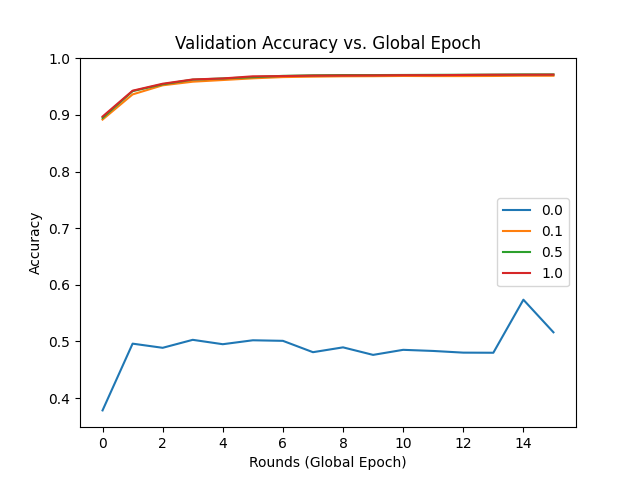
\includegraphics[width=\textwidth]{images/cpreall.png}
    \end{minipage}%
    \begin{minipage}{.5\textwidth}
        \centering
        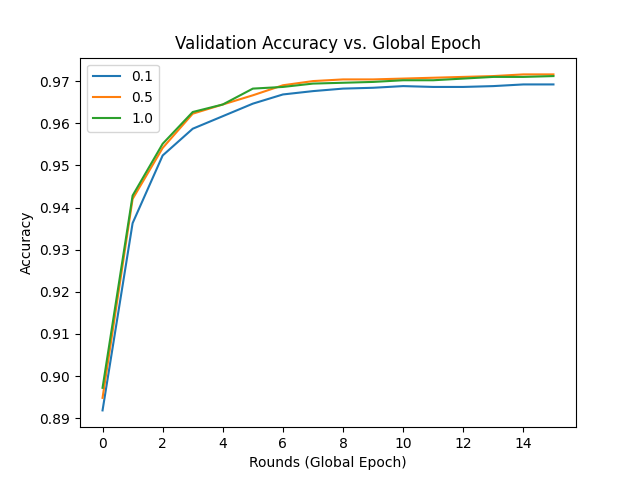
\includegraphics[width=\textwidth]{images/cpretop.png}
    \end{minipage}
    \caption{Accuracy vs. Epoch Plots with Varying $C_{pre}$}
    \label{fig:varycpre}
\end{figure}

However, data standardization proved indispensable in this dataset as accuracy plummets to ~50\% without it.
I tried different learning rates and hyperparameters but to no avail.
Furthermore, using 16-bit floats lead to NaNs without data standardization.

In Figure \ref{fig:varycpre}, I reduced the learning rate to $0.0001$, increased the global epochs to $16$, and experimented with different $C_{pre}$ parameters while keeping the rest constant.
We see that even if only one client shares $\mu_k$ and $\sigma_k$, the accuracy we attain is almost as high as the case in which all clients share standardization data.
However, I don't expect this to be the case when the data is non-IID, which is usually the case in real life.

I fixed $C_{pre}$ to $0.5$ and experimented with different $C$ values.
However, the differences were negligible.

Finally, I tested the model on 10\% of the larger KDD Cup 1999 Data \citep{kdd}, featuring 23 class labels.
Despite the increased size and complexity of the dataset, I still got ~98\% accuracy on the validation set with the single layer linear model, as long as the data standardization step is in-place.


\section{Conclusion}

During this project, I learned a lot about new technologies such as Ethereum, Solidity, and blockchain in general.
I extended my pre-existing machine learning knowledge with federated learning technique.
Although my contribution to federated learning is limited, I did not come across the data standardization stage I devised in the literature, and therefore I think that it might be unique.
I also tackled the problems that arise when federated learning is applied in a blockchain system, such as model size restrictions.
By changing a single configuration parameter, the model size on the blockchain can be halved without any significant impact on accuracy.

Although I started with intrusion detection in mind, the project I developed can be utilized for other blockchain-based federated learning applications easily.
Furthermore, modular platform structure also allows others to develop different blockchain backends for this project.


%% The Appendices part is started with the command \appendix;
%% appendix sections are then done as normal sections
% \appendix
% \section{Sample Appendix Section}

%% If you have bibdatabase file and want bibtex to generate the
%% bibitems, please use
%%
\bibliographystyle{elsarticle-num} 
\bibliography{bib.bib}

%% else use the following coding to input the bibitems directly in the
%% TeX file.

% \begin{thebibliography}{00}

% %% \bibitem{label}
% %% Text of bibliographic item

% \bibitem{}

% \end{thebibliography}
\end{document}
\endinput
%%
%% End of file `elsarticle-template-num.tex'.
